\documentclass[crop,tikz,border=0px,convert=pdf2svg,multi=false]{standalone}
\usepackage{amsfonts}
\usepackage[defaultsans]{opensans}
\usetikzlibrary{shapes,arrows,positioning}
\begin{document}
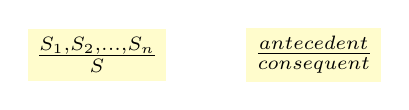
\begin{tikzpicture}[font=\sffamily,
  every node/.style = {draw=none, fill=yellow!20, align=center, inner
    sep=.3em, text centered}]

  \node (n0) {\(\frac{S_1, S_2, \dots, S_n}{S}\)};
  \node [right=of n0] {\(\frac{antecedent}{consequent}\)};

\end{tikzpicture}
\end{document}
